\chapter{Results, Validation, and Discussion}
\label{chapter:results}

\section{Tree Genus Classification}

The results shown in Fig.\,\ref{fig:class_analysis} were obtained using the best model developed in Chapter\,\ref{chapter:hyper}. The metrics were calculated using 10,000 validation samples. As illustrated, tree genera with approximately 20,000 occurrences exhibited poorer classification performance compared to those genera with a larger number of training samples. This trend is further supported by a positive correlation between the number of training samples and the performance metrics, indicating that genera with more extensive training data achieve higher classification accuracy.

\begin{figure}[ht]
    \centering
    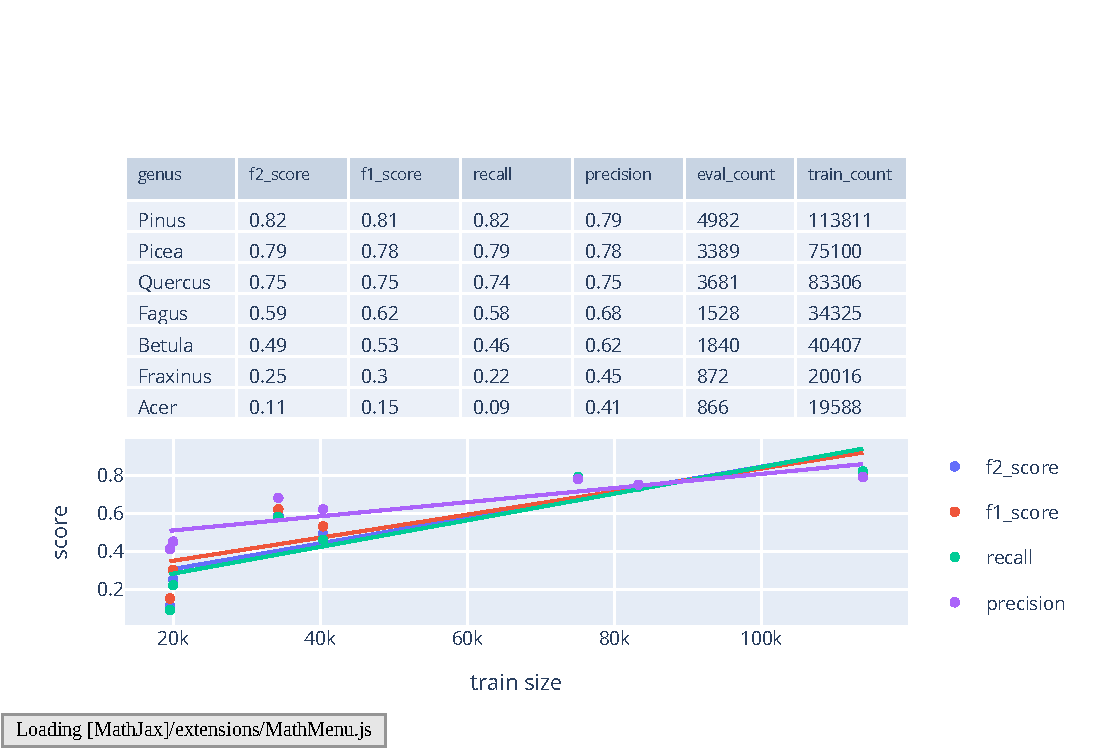
\includegraphics[width=0.98\linewidth, trim={10pt 20pt 10pt 40pt}, clip]{figures/figures_class/class_analysis.pdf}
    \caption{Top: table displaying the evaluation metrics, including evaluation count and training count, for each tree genus. Bottom: scatter plot of the scores with a respective ordinary least squares (OLS) fit line.}
    \label{fig:class_analysis}
\end{figure}

The poor performance observed for certain tree genera, as indicated by low scores, can largely be attributed to class imbalance within the dataset. Genera with fewer occurrences, especially those with around 20,000 occurrences or fewer, are underrepresented during model training. This limited exposure hinders the model's ability to learn and accurately classify these less common genera. Additionally, when multiple genera are present within a single sample, the spectral signatures of the less dominant genera may be overshadowed, making it more challenging for the model to distinguish them effectively.

Furthermore, the underperforming genera might require additional or different features that are not fully captured by the current model. The overlap in spectral features among different genera can further complicate accurate classification, especially when the less common genera make up only a small portion of the sample area. Addressing these challenges may involve strategies such as increasing the dataset size, applying data augmentation techniques, or developing specialized models tailored to these underrepresented classes. It is worth noting that simply duplicating samples of underperforming genera may exacerbate the problem, given that these samples often contain multiple genera.

\section{Change Map Correlations}

\begin{figure}[ht]
    \centering
    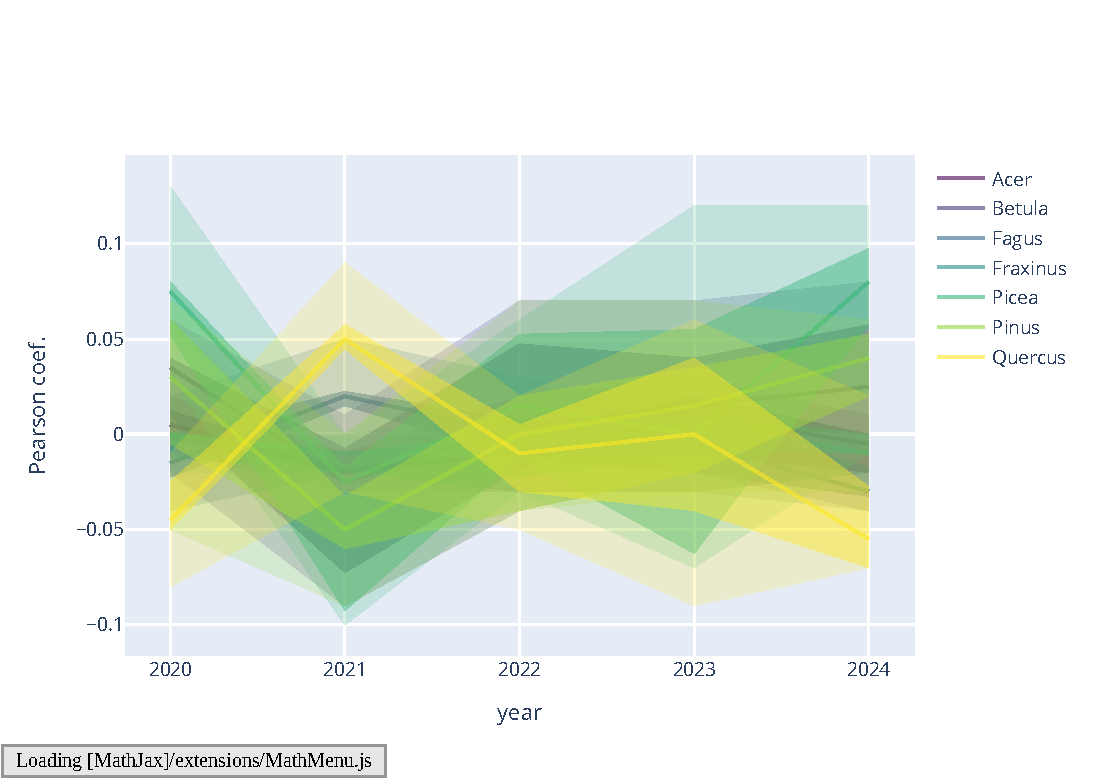
\includegraphics[width=0.98\linewidth, trim={10pt 20pt 10pt 40pt}, clip]{figures/figures_climate/genus_corr.pdf}
    \caption{Median and quantiles of Pearson correlations between changes in tree genera maps predicted by classification and differences in meteorological conditions.}
    \label{fig:genus_corr}
\end{figure}

The differences between the representative medians (Fig.\,\ref{fig:selected_variables_stats}) and those for each individual year from 2020 to 2024 were analyzed and correlated with the discrepancies between classification genera predictions and actual values. These results are summarized in Fig.\,\ref{fig:genus_corr}. 

Fig.\,\ref{fig:genus_corr} suggests that, over a short-term period of 5 years, the 7 most prominent European tree genera were not significantly affected by climate change. However, this does not account for potential long-term impacts, where even small changes could have substantial effects on ecological dynamics. Additionally, this analysis is limited to Europe, a region that may experience less pronounced climate changes compared to other parts of the world, as discussed in \cite{hoegh2018climate}. Furthermore, the study does not consider less common tree genera, which might be more sensitive to climate change and could exhibit different patterns of response.

\section{Relationship Modeling}

Unlike correlation, which measures the strength and direction of linear relationships between variables, relationship modeling with neural networks aims to uncover complex, non-linear interactions between variables. To further explore the relationships illustrated in Fig.\,\ref{fig:genus_corr}, a narrow, fully-connected regression neural network was developed. This network used changes in meteorological variables as predictors to analyze how these changes relate to variations in tree genera maps.

A model was trained using the Huber loss function, which combines the advantages of Mean Absolute Error (MAE) and Mean Squared Error (MSE). Huber loss was chosen due to its effectiveness in scenarios with noisy data and outliers, as it provides a balance between the robustness of MAE and the sensitivity to errors of MSE. 

R$^2$ was used as a primary metric because it directly measures the proportion of variance in the dependent variable that can be explained by the independent variables. This metric is particularly valuable for assessing how well the model captures the underlying relationships in the data. A higher R$^2$ value indicates a stronger relationship between the predictors and the target variable, offering insights into the effectiveness of the model in explaining variability.

MAE was chosen to evaluate the accuracy of the model's predictions. MAE provides an average of the absolute differences between the predicted and actual values, giving a clear indication of the magnitude of prediction errors. While MAE does not measure the strength of relationships directly, it helps assess how closely the model's predictions align with actual outcomes.


\begin{figure}[ht]
    \centering
    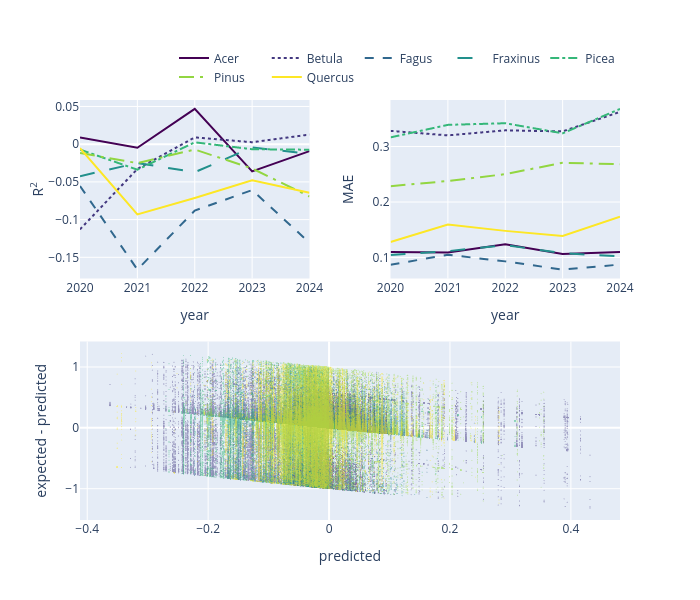
\includegraphics[width=0.98\linewidth, trim={10pt 20pt 50pt 40pt}, clip]{figures/figures_climate/regression_results.png}
    \caption{R$^2$ score (top-left), MAE (top-right), and residuals (bottom) for a narrow, fully-connected regression neural network, using meteorological change maps as predictors for changes in tree genus maps derived from tree classification.}
    \label{fig:regression_results}
\end{figure}

As illustrated in Fig.\,\ref{fig:regression_results}, the model exhibits a very low, and at times negative, R$^2$ value along with a high MAE. Additionally, a random sample of 50,000 residuals for the year 2024 do not display a discernible pattern, aside from clustering that reflects the original data being naturally grouped into true and false values. These results collectively indicate that the model fails to capture any significant relationship between the climate change maps and the changes in tree genus distributions. The poor performance metrics suggest that the predictors used do not meaningfully account for the variability in tree genus changes as a function of the climate variables used in this study.